\section{Arrays and data structures}
Data structures is one of the main concept in computer science, even in this course we have already talk about it (the stack).\\
\begin{parag}{Arrays in high-level languages}
	\begin{lstlisting}[language=Scala]
val myData: Array[Short] = Array(10407, -16533, -22715, 123133, 12512)
    \end{lstlisting}
\end{parag}
Here we have a sequence of number that are indexed, the question however is how do we store them.\\
We have a lot of ways to do so (three), we can have a pointer to the first element, and the having the other following this one. With this methode the issue is when does the array stops?\\
One way to do so is to put a \textit{null} element at the end of the array so that we know that this is the end of the array.  The definition of string are in fact an array of char with the 0 char at the end.\\
Another way with this is just to to do nothing. Having a pointer to the start of the array and the hoping t hat the programmer knows what is his doing. \texttt{C} Arrays for instance are built like this.\\
A whole other way is to have, at the start of the array the length of the array. You have a pointer at the start of the array which is the length of the array and then you do your computing as usual
\begin{center}
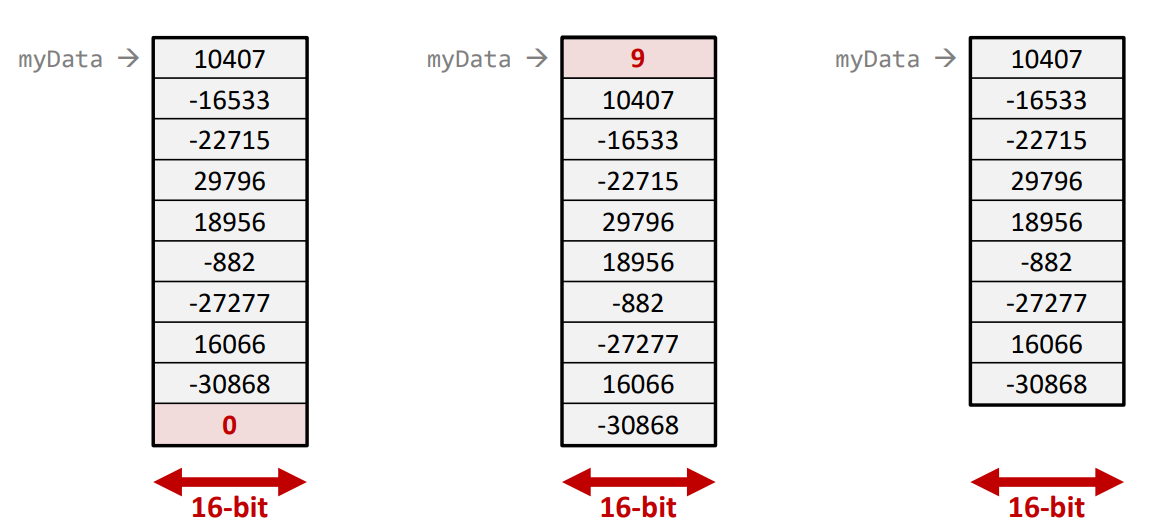
\includegraphics[scale=0.3]{screenshots/2025-10-21.png}
\end{center}
\begin{parag}{Adding Positive elements}
    To add all the positie elements in an array of signed 16-bit integers we would:
	\begin{itemize}
	    \item At call time, \texttt{a0} points to the array (and, in type 3, \texttt{a1} is the length)
	    \item At return time, \texttt{a0} contain the result
	\end{itemize}
	The result for the type 3 (written in \texttt{c}):
	\begin{lstlisting}[language=c]
short add_positive(short myData[], int N) {
	short  sum = 0;
	for (int i = 0; i < N; i++) {
		if (myData[i] > 0) {
			sum += myData[i];
		}
	}
	return sum;
}
	\end{lstlisting}
\end{parag}
\begin{parag}{Adding positive elements (Type 1)}
    For the first type let us write the code for this in RISC-V:
	\begin{lstlisting}[language={[RISC-V]Assembler}]
add_positive:
	li t0, 0  #t0 will hold the sum (initialized to 0)

next_short:
	lh t1, 0(a0) # Load short (half-word) at address a0 into t1
	beqz t1, end  # If t1 is 0 (null short) we are done
	bltz t1, negative  # if t1 is negative ignore
	add t0, t0, t1  #Add t1 to the sum (t0)

negative:
	addi a0, a0, 2  # move array pointer (a0) by sizeof(short) to the next element
	j next_short  # repeat the loop
end:
	mv a0, t0  # move the sum (t0) into a0 as the return value
	ret # Return the caller
	\end{lstlisting}
	
	
\end{parag}

\begin{parag}{Adding positive element Type 2}
	\begin{lstlisting}[language={[RISC-V]Assembler}]
addi_positive:
	li 01, 0 #t0 will hold the sum (initialized to 0)
	lh t1, 0(a0) # t1 will count the elemetnts to process
	add a0, a0, 2  # Move array pointer (a0) to the first real element

next_short:
	beqz t1, end  # If t1 is 0 (no more elements), we are done
	lh t2, 0(a0) # Load short (half-word) at address a0 into t2
	bltz t2, negative # If t2 is negative, ignore
	add t0, t0 t2  # Add t2 to the sum (t0)

negative:
	addi a0, a0, 2 # Move array pointer (a0) by sizeof(short)
	addi t1, t1, -1 # Decrement the counter of elements to process
	j next_short  # repeat the loop
end:
	mv a0, t0 # Move the sum (t0) into a0 as the return value
	ret # Return to caller
\end{lstlisting}

\end{parag}



\begin{parag}{Adding positive element Type 3}
	\begin{lstlisting}[language={[RISC-V]Assembler}]
addi_positive:
	li 01, 0 #t0 will hold the sum (initialized to 0)
	mv t1, a1 # t1 will count the elemnts to process (a1)

next_short:
	beqz t1, end  # If t1 is 0 (no more elements), we are done
	lh t2, 0(a0) # Load short (half-word) at address a0 into t2
	bltz t2, negative # If t2 is negative, ignore
	add t0, t0 t2  # Add t2 to the sum (t0)

negative:
	addi a0, a0, 2 # Move array pointer (a0) by sizeof(short)
	addi t1, t1, -1 # Decrement the counter of elements to process
	j next_short  # repeat the loop
end:
	mv a0, t0 # Move the sum (t0) into a0 as the return value
	ret # Return to caller
\end{lstlisting}

\end{parag}

\begin{parag}{Adding positive elements (variation on c)}
	Let us add positive elements in an array of signed 16-bits integers:
	\begin{itemize}
	    \item At call time, \texttt{a0} points to the arrays and \texttt{a1} is the length of the arr
	    \item At return time \texttt{a0} contains the result
	\end{itemize}
	Write it by incrementing the index of the array:\\
	\begin{lstlisting}[language=c]
int i = 0;
while (i < N) {
	if (myData[i] > 0) {
		...
	}
	i++
}
	\end{lstlisting}
	This is equivalent to:
	\begin{lstlisting}[language=c]
int i;
for (i = 0; i < n; i++) {
	if (myData[i] > 0) {
		...
	}
}
	\end{lstlisting}
	
	Here we see that we have a variable \texttt{i}  which is incremented by one, therefore, the way of doing this if we were to be compiled would be by having a variable that is incremented by 1 in very loop \textbf{then} be multiplied by the sizeof the data (2 bytes).
	\begin{lstlisting}[language={[RISC-V]Assembler}]
addi_positive:
	li t0, 0 #t0 will hold the sum (initialized to 0)
	mv t1, 0 # t1 will hold the array index

next_index:
	beqz t1, end  # If index >= number of elements , we are done
	slli t2, t1, 1  # t2 = offset of the element as index (t1) * sizeof(short)
	add t2, a0, t2 # Address of the element = myData (a0) + offset(t2)
	lh t3, 0(t2) # load short (half-word) at address a0 into t3
	bltz t3, negative #if t3 is negative, ignore
	add t0, t0, t3 # Add t3, to the sum (t0)

negativ:
	addi t1, t1, 1 #Increment the counter of element to process
	j next_index  # repeat the loop
end:
	mv a0, t0 # Move the sum (t0) into a0 as the return value
	ret # Return to caller
	\end{lstlisting}
	
	\begin{subparag}{Which is better}
	    We have now two different way to do the same type (type 3), however which one is faster? this question can be easily answers: the first one that we have written has less intrustion $\implies$ faster. (this is not always that simple)\\
		But this points out an issue, we need \important{good compiler}, we need a compiler that can translated our code into the fastest assembly possible.
	\end{subparag}
\end{parag}


\begin{parag}{Linked list}
    Another way to store data is with a linked list:
	\begin{center}
	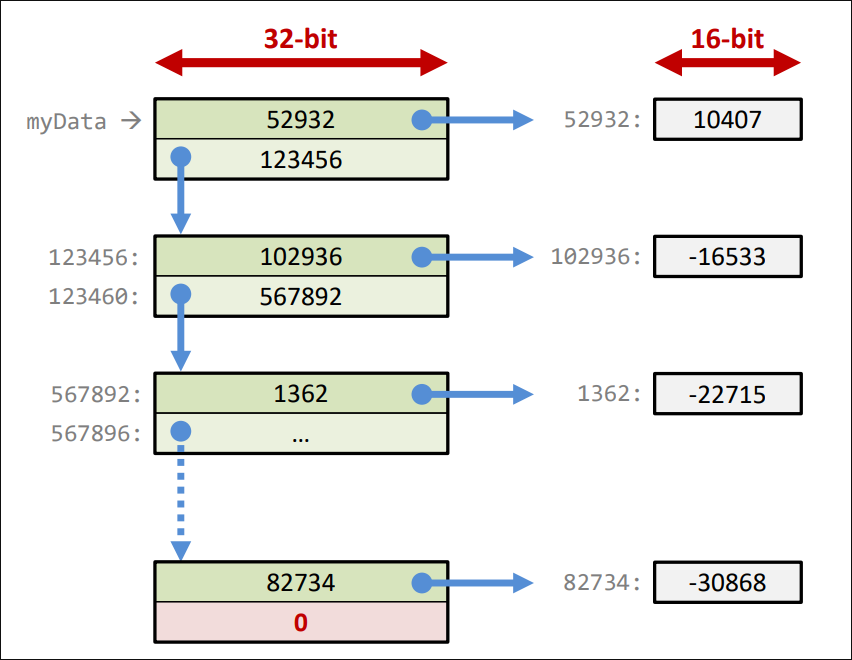
\includegraphics[scale=0.3]{screenshots/2025-10-21_1.png}
	\end{center}
	As we can see here this is the same principle as what we did before, we store for each element the current address of the value \important{and} the address of the next value. To  iterate through this list all we have to do is to go to the current value get the value via the address and then take the next iteration with the second address.\\
	What is good about this is that:
	\begin{itemize}
	    \item  Insert element in the array is very easy
	\end{itemize}
	However there is a lot of bad thing here:
	\begin{itemize}
	    \item For each value we have to use 64 bits of addresses which is a lot 
		\item iterate through the list seems nice however are all the instruction truly equal?	
	\end{itemize}
	For  instance imagine we wanted to recreate the same code as the one we wrote for the other arrays:
	\begin{lstlisting}[language={[RISC-V]Assembler}]
add_positive:
	li t0, 0 # t0 will hold the sum
next_element:
	beqz a0, end # If address of next element (a0) is zero, we are done
	lw t1, 0(a0) # Load address of actual data into t1
	lh t1, 0(t1) # Load short (half-word) at address t1 into t1
	bltz t1, negative # if t1 is negative, ignore 
	add t0, t0, t1  #  Add t1 to the sum (t0)

negative:
	lw a0, 4(a0) # Load address of next element into a0
	j next_index
end: 
	mv a0, t0 # Move the sum (t0) into a0 as the return value
	ret # Return to caller
	\end{lstlisting}
	
	As we can see here: this is not much more complex. but is it more efficient: no. The instruction of loading and storing are way slower than the other instruction, the fact that this way of computing leads to a lot more of load makes it way slower.
	
	
\end{parag}






